\chapter{The DarkSide experiment}
\label{ch:darkside}

The DarkSide20k experiment is a planned dual phase liquid argon (LAr) time
projection chamber (TPC) designed to detect nuclear recoils (NR) with energy in
the range \SI{30}{keV} to \SI{200}{keV}, with a 20 metric ton fiducial target
mass, which with 5 years of exposure should reach a sensitivity of
\SI{1.2e-48}{cm^2} on the spin-independent (SI) WIMP-nucleon cross section at
WIMP mass \SI{1}{TeV}, to be compared with the current best limit
\SI{1e-46}{cm^2} by XENON1T. DarkSide20k is optimized for high WIMP masses.

The project was born joining the forces of four LAr dark matter search
experiments: ArDM, DarkSide-50, DEAP-3600 and MiniCLEAN. It will be hosted by
Laboratori Nazionali del Gran Sasso (LNGS). We give here a brief description of
the experiment. For details, see the published ``Yellow Book''
\cite{aalseth2018}. An unpublished but publicly available preliminary design
report \cite{aalseth2019} provides more up to date information, in particular
the veto system was completely redesigned.

\section{Pulse shape discrimination}

When radiation hits an argon atom, the release of energy produces ions, and
excited states which decay emitting ultraviolet photons. See
\cite[sec.~3.1]{luzzi2020} for a detailed explanation of the chain of
reactions. What matters is that:
%
\begin{enumerate}
    
    \item the relative amount of ionization and photons produced is different
    if the incoming particle scatters on an electron or a nucleus;
    
    \item the photons are produced by two possible excited states, one with
    a fast decay constant, \SI{7}{ns}, and a slow one with \SI{1.6}{\micro s};
    
    \item the relative amount of fast and slow photons is different for
    electron recoil (ER, 1 to 3) and nuclear recoil (NR, 3 to 1).
    
\end{enumerate}

Property~(3) is the most important. Discriminating ER from NR using the
fast/slow ratio is called pulse shape discrimination (PSD).

To reach the required sensitivity, it is necessary for the experiment to have
zero background, in the sense that all background radiations must be identified
and removed from the data instead of accounted for with a model. To get an idea
why, consider that if a detector does not observe any signal for a time $t$ on
$n$ targets, the upper bound on the interaction probability goes down like
$1/(nt)$. Instead, if there is a background rate $r$, the uncertainty is
dominated by the Poisson error and goes like $1/\sqrt{rnt}$.

The collaborations did not find a way to eliminate the backgrounds from beta
and gamma rays producing ER, while it is feasible to identify or exclude the
neutrons producing NR. This is the reason why these experiments study nuclear
recoils and need to distinguish between NR and ER. In the planned exposure of
\SI{100}{t yr} of DarkSide20k, less than 0.1 background events are expected.

An irreducible background is given by neutrinos, which are indistinguishable
from WIMPs without directional information. When the ``neutrino floor'' will be
reached (see \autoref{fig:sigmalimits}), the experiments will at least do some
new measurements on solar neutrinos, if dark matter is not found. DarkSide20k
expects approximately one neutrino recoil.

For comparison, in xenon detectors the PSD is not effective, and the most
important discriminant is the light/ionization ratio.

\section{Dual phase TPC}

\begin{figure}
    
    \widecenter{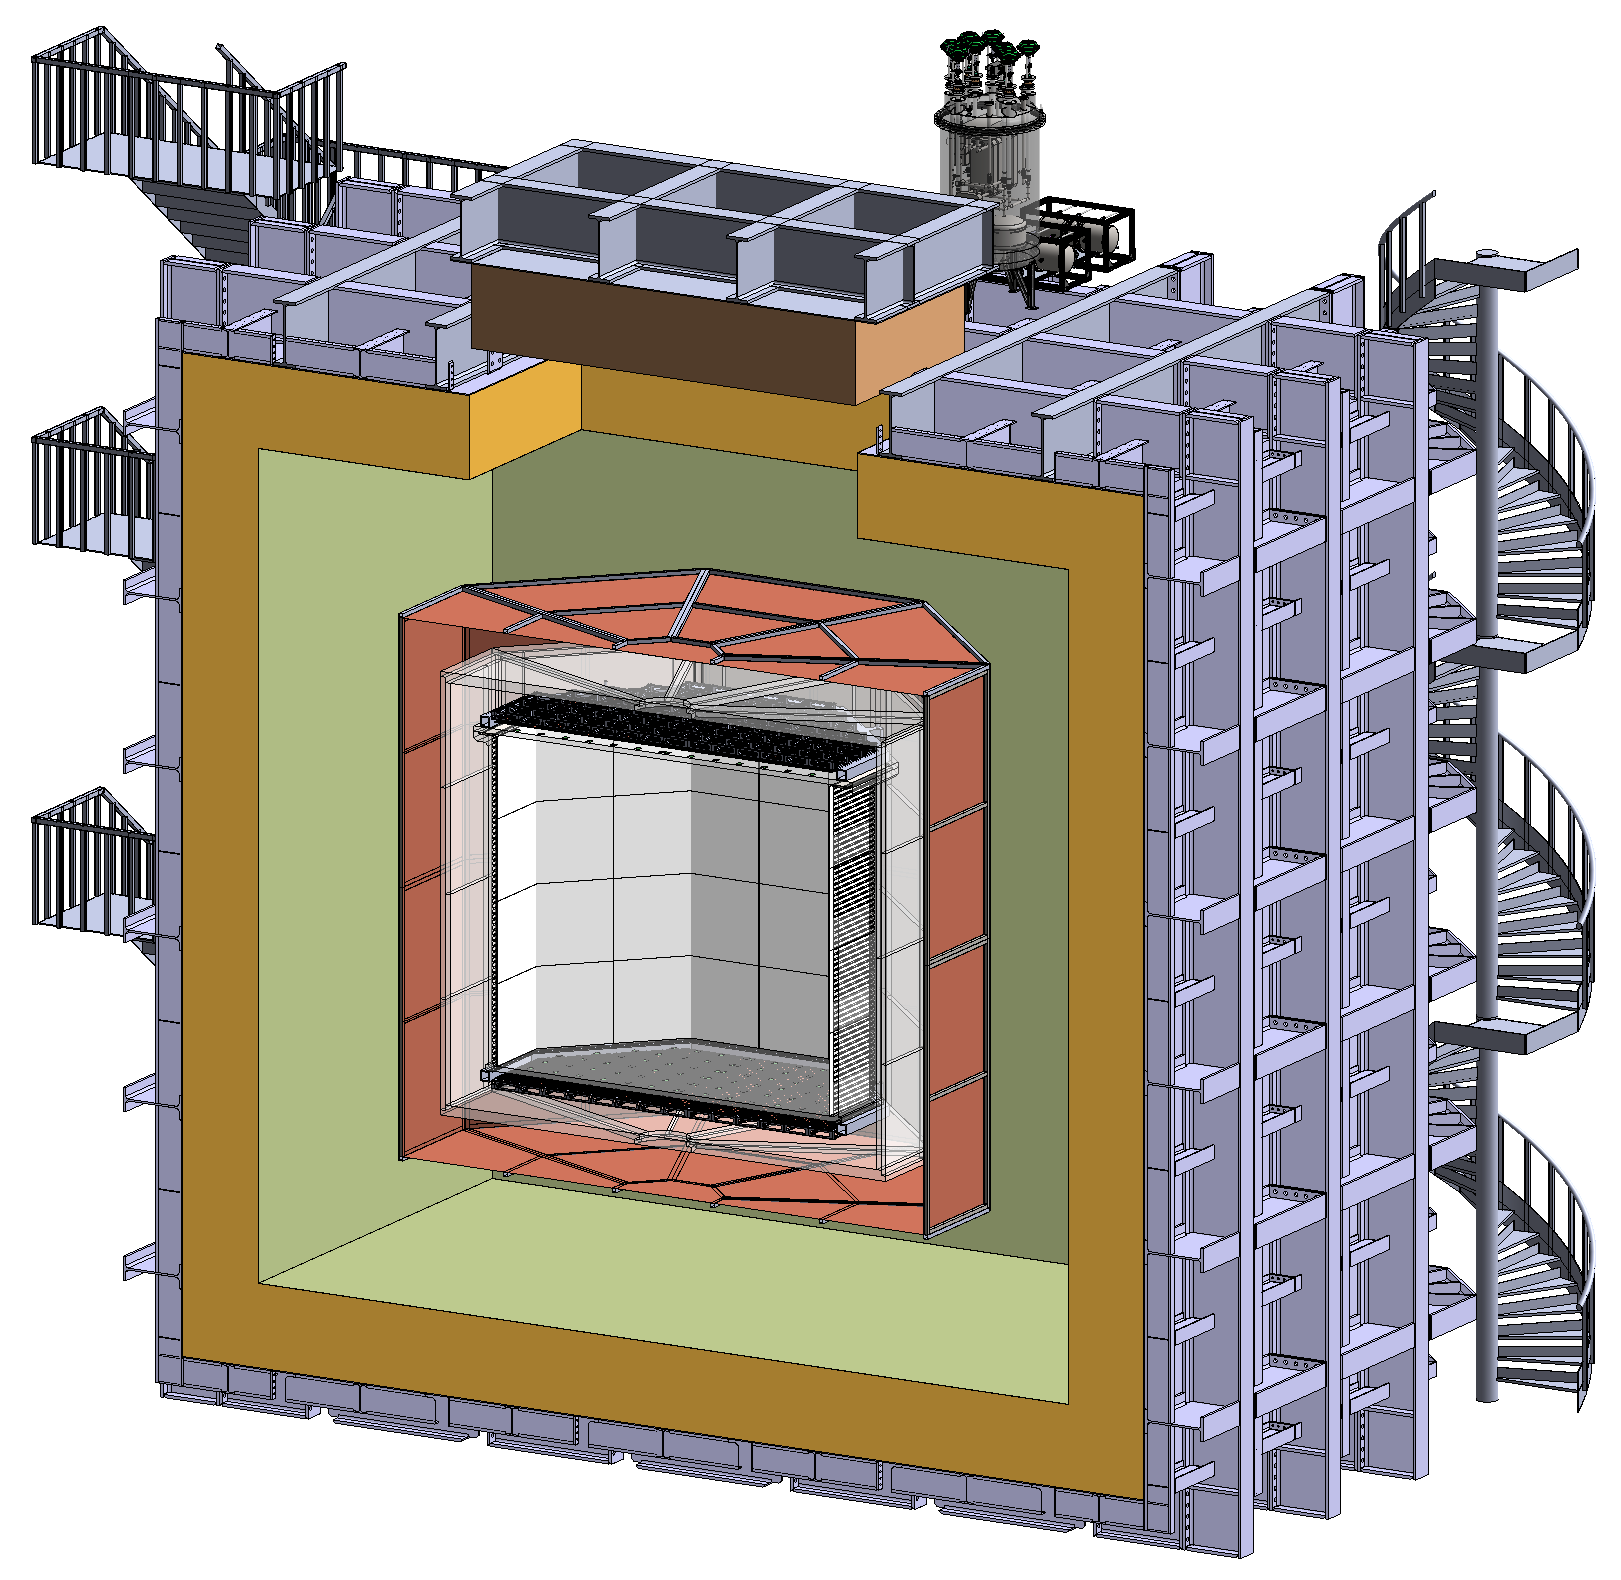
\includegraphics[width=\textwidth]{darkside20k}}
    
    \caption{\label{fig:darkside20k} Scheme of DarkSide20k. From
    \cite[2]{aalseth2019}. The innermost cylinder is the TPC, wrapped in the
    two layers of the veto detector. The outer container is the cryostat,
    copied from the ProtoDune experiment.}
    
\end{figure}

In principle the mass of argon could be surrounded with photodetectors which
count the photons produced by the recoils. This would be sufficient to
implement the PSD.

However, this would not allow to reconstruct precisely and reliably the
position of the signal. The position information is used to reject two kinds of
backgrounds: 1)~backgrounds producing multiple hits, considering that a WIMP
would scatter just once, and 2)~backgrounds on the border of the target,
produced by the radioactive contamination of the materials of the detector.

To measure the position, a time projection chamber (TPC) is employed. The argon
is put into a cylinder, about \SI{2.5}{m} tall and \SI{3}{m} wide, where an
uniform \SI{200}{V/cm} electric field pointing downward is maintained. The free
electrons produced by ionization drift upward, taking at most \SI{4}{\micro s}
from the bottom to the top of the cylinder, while the photons reach immediately
the photodetectors, placed on the top and bottom faces.

On the top of the cylinder, just below the photodetectors, a ``pocket'' facing
downward is kept filled with gaseous argon, like a diving bell. An additional
grid imposes an higher electric field in the gaseous phase, called ``extraction
field''. When the electrons emerge from the liquid phase, they are accelerated
toward the anode and scintillate the argon vapor. The extraction field is not
intense enough to induce further ionization when the electrons pass, so the
information on the number of ionized electrons is preserved. This scintillation
light hits the top photodetection plane concentrated in a narrow spot.

The prompt photons produced by the recoil are called S1, while the light
emitted by extracted electrons S2. The names stand for ``first signal'' and
``second signal'', since S2 arrives after S1 due to the drift time. This delay
allows to deduce the depth of the recoil, the $z$ coordinate. Since the S2
light is concentrated, it is easy to measure its position on the horizontal
plane. The electrons drift vertically, so this matches the $xy$ coordinates
of the recoil. Thus the TPC permits a 3D reconstruction of the signals.

\autoref{fig:darkside20k} shows a scheme of DarkSide20k. The innermost cylinder
is the TPC. The two successive shells delimit two layers of LAr which are used
as target for the veto detector. Cosmic rays can produce neutrons when they hit
the detector, but first they have to pass through the veto detector, which
tells the system to ignore the signal.

The outermost tank is the cryostat, which is completely filled with LAr. The
argon circuit of the TPC is separate, because it is filled with argon extracted
underground (UAr) and purified to have about 1/1400 the amount of radioactive
$^{39}$Ar isotope relative to argon distilled from the atmosphere (AAr), which
is used for the rest of the system.

\section{Photodetectors}

\begin{figure}
    
    \widecenter{
        \newlength\sipmheight
        \setlength\sipmheight{5cm}
        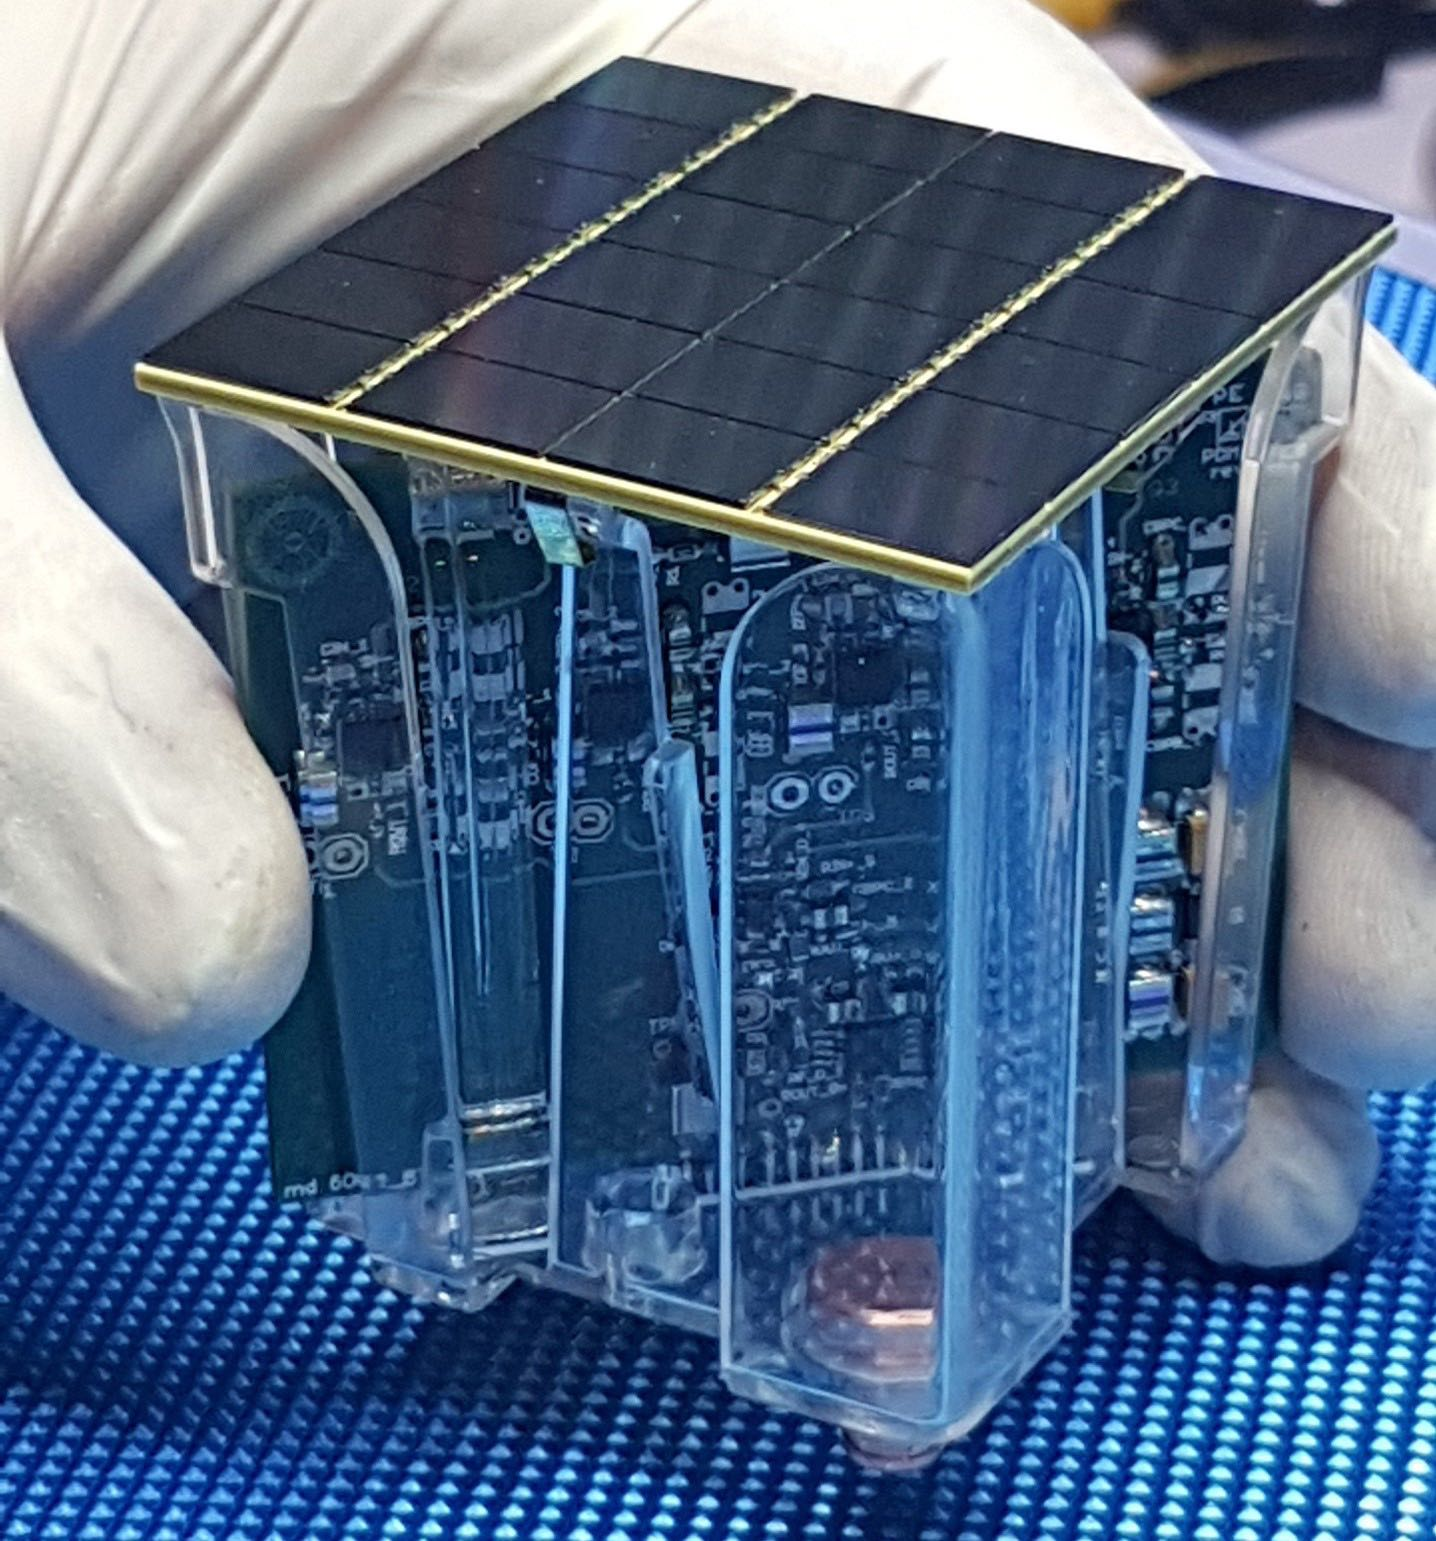
\includegraphics[height=\sipmheight]{sipm1}
        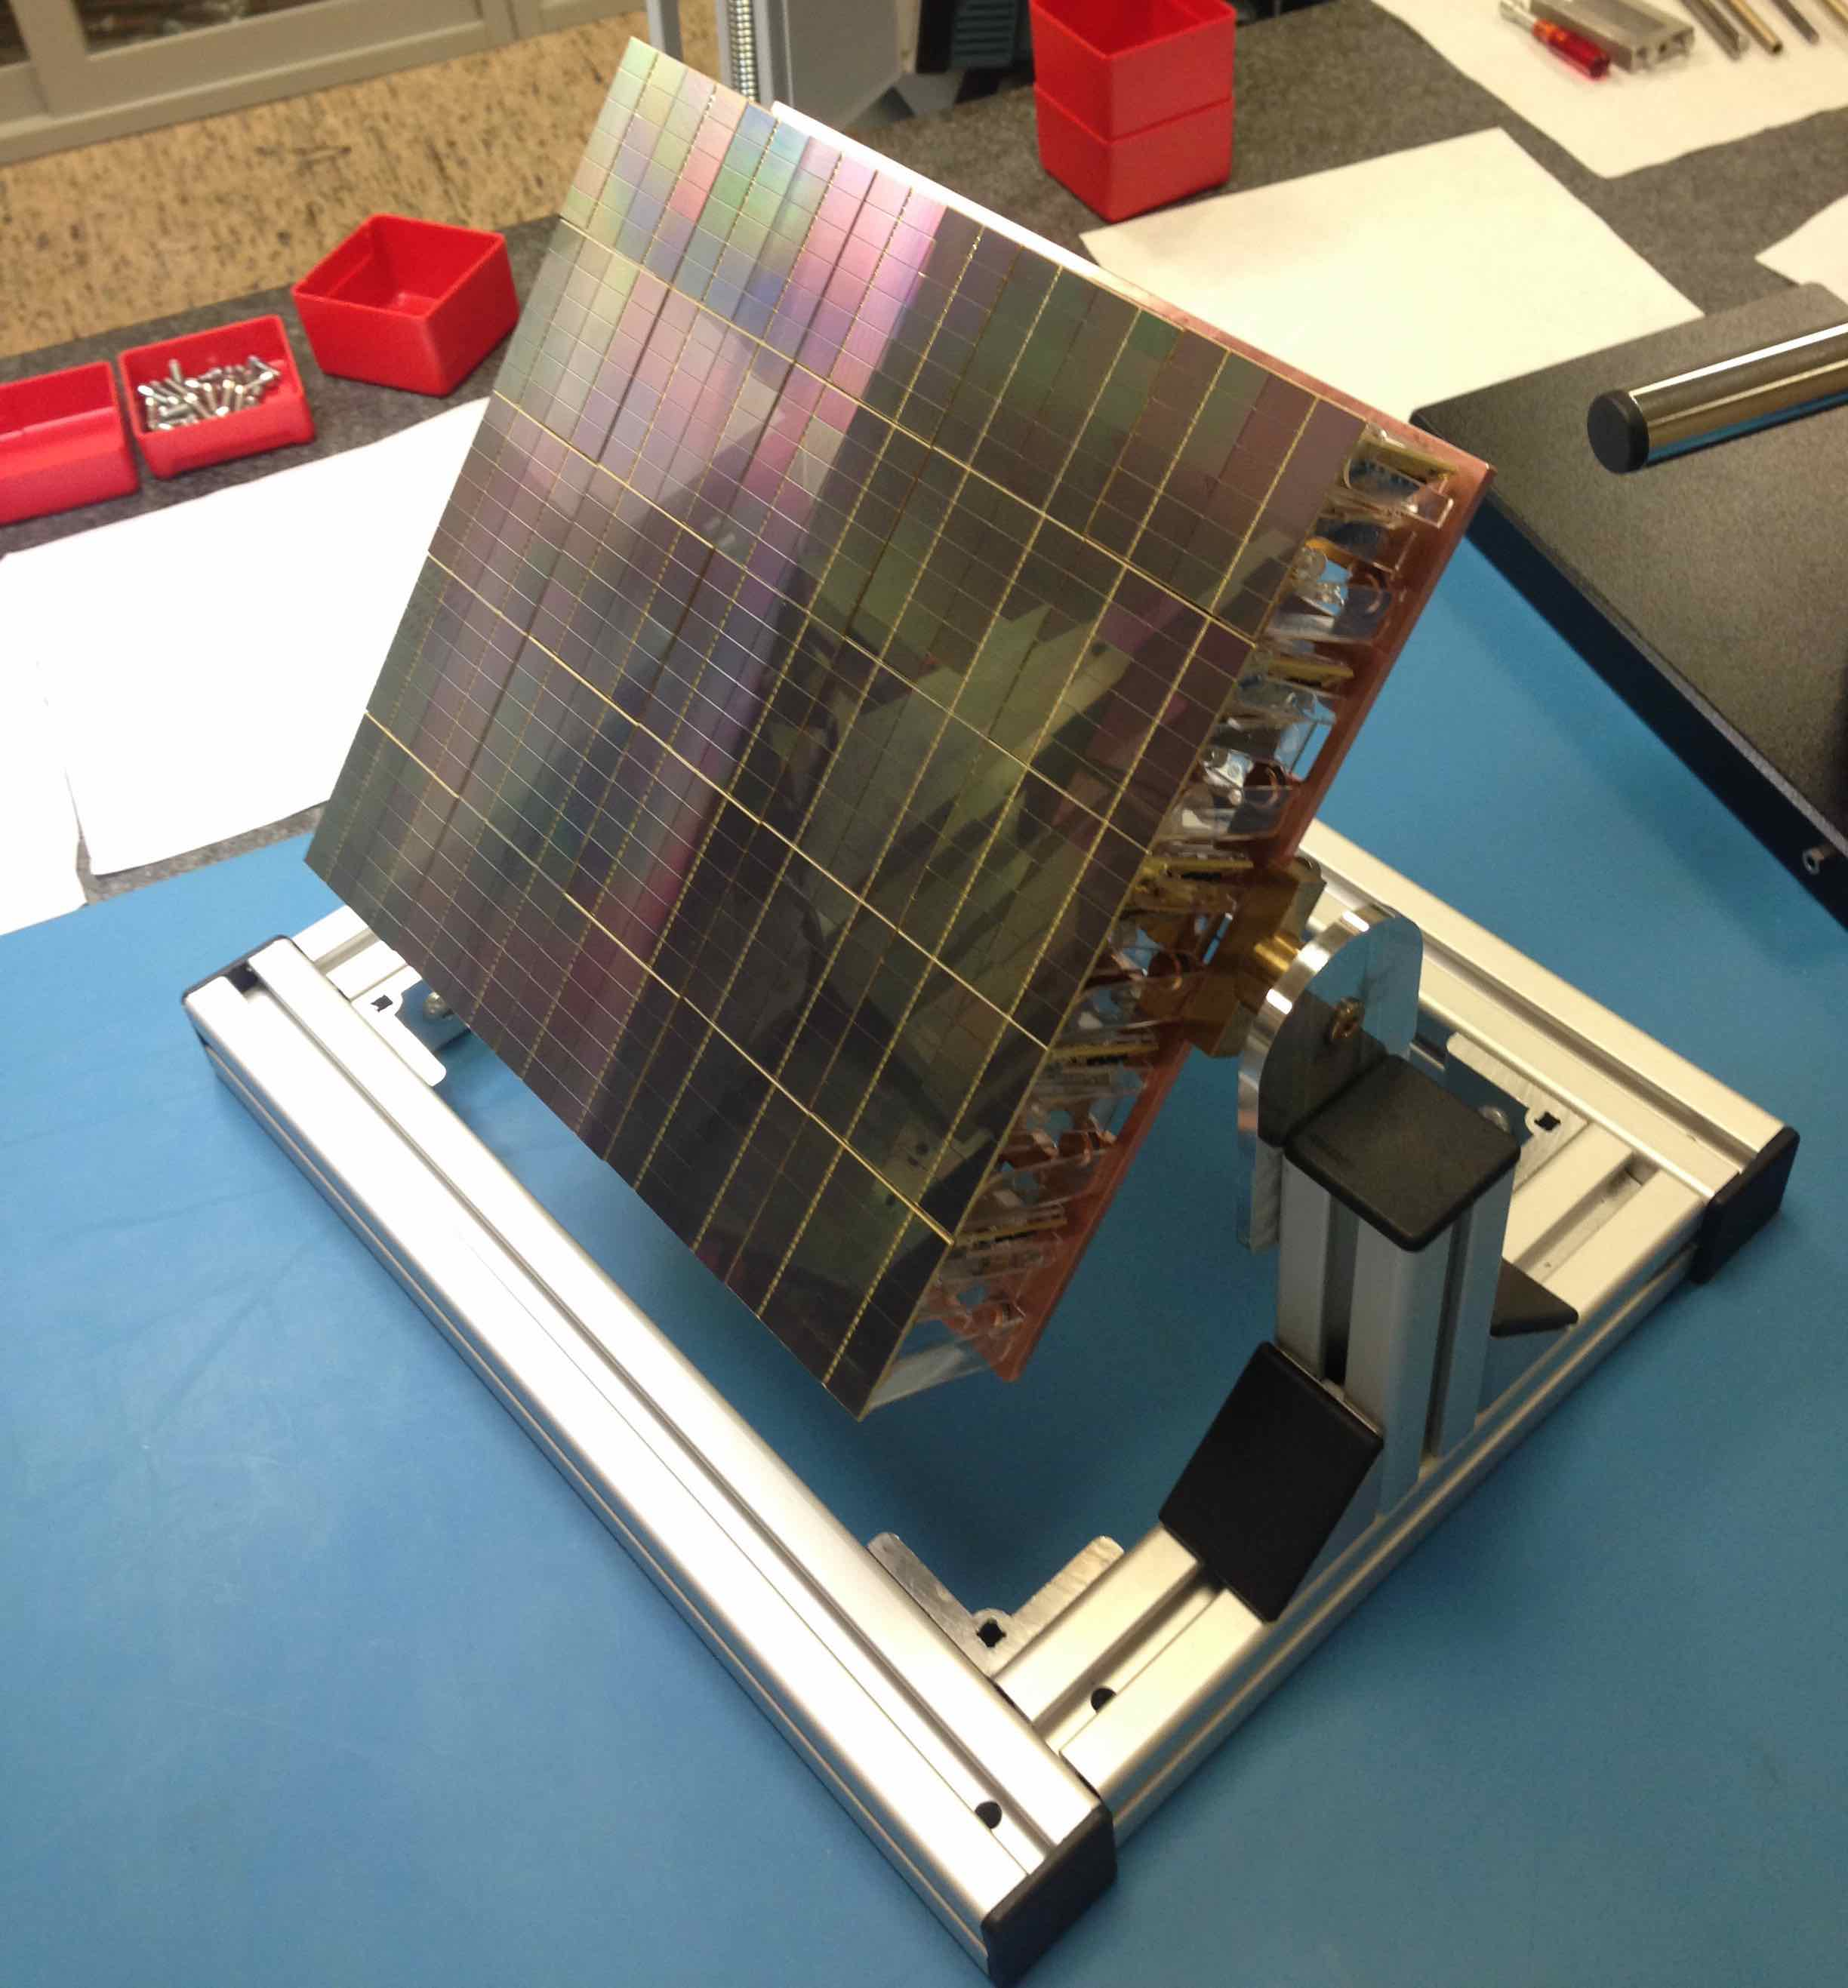
\includegraphics[height=\sipmheight]{sipm2}
    }
    
    \caption{\label{fig:sipm} Left panel: a photodetector module (PDM). Right
    panel: a motherboard with 25 PDMs. From \cite[4]{aalseth2019}.}
    
\end{figure}

\stracka{Descrizione fotoelettronica: puoi trarre cospicua ispirazione dalla
tesi del Marasciulli
%
https://etd.adm.unipi.it/t/etd-09252019-101839/ 
%
E' in italiano e comunque dovrai sintetizzare per fare diventare quello che lui
mette come capitolo a parte (il 4) in una sezione del tuo cap. 2. Per esempio,
a te sicuramente non interessano le descrizioni dei coperchi delle custodie
delle Tile (mentre a lui sì: per lui il focus era la PE).
%
Nel Cap.5 poi lui parla di diversi test e della prima MB. Tu invece usi MB2, e
sta sopra in Proto0 (non sotto come nel caso di Andrea). Giusto per non fare
confusione nel caso volessi prendere qualche figura da qui: c'è da fare
attenzione.
%
Qui raccogli anche le varie cose che al momento sono spesso scritte dopo il
punto in cui ti servono per la prima volta.}

\marginpar{controllare che quando richiamo le cose sulla DAQ le cose che dico
sono anche nel capitolo 2, e linkare\\
separare descrizione tile e pdm\\
aggiungere figura tile da marasciulli\\
ftoto della feb con le scrtiitne 4.14, speiegare meglio i collegamenti\\
pdu ha il transmission module + steering module (quello che alimenta e
disabilita le singole tile)\\
chiarire che i pdm della pdu sono gestiti insieme\\
verificare che la descrizione dello SPAD nel capitolo 7 sia giusta, c'è scritto
nel marasciulli\\
spiegare chiaramente che i WIMP sono supposti fare urto elastico o sui nuclei o
sugli elettroni}

DarkSide50 uses photomultiplier tubes (PMTs) for photodetection. DarkSide20k
instead will be equipped with silicon photomultipliers (SiPMs). The SiPMs are
large matrices of photodiodes connected in parallel and operated in Geiger
mode. The advantages of SiPMs compared to PMTs are:
%
\begin{itemize}
    
    \item single photon resolution;
    
    \item higher filling factor, i.e., they tile more densely the surface;
    
    \item low voltage bias;
    
    \item better radio-purity;
    
    \item higher photon detection efficiency (PDE).

\end{itemize}

The basic unit of the photodetection system is the photodetector module (PDM),
consisting in a Tile, i.e., a $6\times 4$ matrix of SiPMs totaling
\SI{25}{cm^2}, connected to a front end board (FEB) hosting the biasing circuit
and the preamplifier. Matrices of $5\times 5$ PDMs are bound together to form a
motherboard (MB). Each motherboard is paired with transmission electronics
forming a photodetector unit (PDU). \autoref{fig:sipm} shows a PDM and a MB.

\marginpar{Da qualche parte devo definire l'overvoltage}

In the PDM the SiPMs are connected in parallel branches of two SiPMs in series
each. This increases the noise compared to having a preamplifier for each SiPM,
but is necessary because the electronic components are a source of radioactive
contamination, and because the power dissipated by the amplifiers increases the
temperature.

\stracka{ocio: prima dici che sono connessi in parallelo, ma quando si passa
dal SiPM alla Tile, hai configurazioni più complicate: somme di 4 settori,
ognuno dei quali combina in parallelo 3 serie di 2 SiPM (come dici da qualche
parte dopo). Questo chiariscilo in Cap.2}

The signals are carried out of the cryostat to digitizer boards equipped with
14~bit \SI{125}{MSa/s} ADCs connected to an FPGA and a controller CPU. The
digitizer board is expected to implement basic single photon pulse
identification and send selected data through an ethernet link to a front end
processor (FEP), a normal CPU station, that refines the analysis. Finally, an
event builder farm takes the information from all the FEPs, divides the sets of
photon hits into events, and decides what to record to permanent storage.

\marginpar{nel capitolo 2 spiegare che i sipm hanno i rumori, così introduco la
mia tesi}
